\section{Programmstruktur}\label{sec:scope}
Dieser Abschnitt behandelt die strukturellen Unterschiede von Java- und COBOL-Programmen. Dazu wird auf den Scope von Variablen eingegangen und erläutert in welche Einheiten sich die Programme der jeweiligen Sprache aufteilen lassen. Der sog. Scope, zu deutsch Gültigkeitsbereich, gibt in der Programmierung an, in welchem Bereich eine Variable gültig ist. \todo{enum, interfaces irgendwo einbauen}

\subsection*{Java}

\subsubsection*{Scope}
In Java ist der Scope einer Variablen meist einfach zu erkennen. Eine Variable ist innerhalb der geschweiften Klammern gültig, die die Variablendeklaration beinhalten. Dies verdeutlicht \autoref{javaScope}.\\

Die Variable \mintinline{java}{memberVariable} ist innerhalb der gesamten Klasse \mintinline{java}{ScopeExample}, also in jeder enthaltenen Methode, verschachtelten Klassen und wiederum deren Methoden, gültig. Eine Variable mit selbem Namen kann auch innerhalb einer Methode deklariert werden. Auf die Instanzvariable kann mit dem \mintinline{java}{this}-Schlüsselwort zugegriffen werden. In geschachtelten Klassen muss zusätzlich der Klassenname vorangestellt werden wie Zeile 27 zeigt.  Ist keine lokale Variable mit selbem Namen vorhanden, so kann dieses Schlüsselwort auch weggelassen werden. \\

Wie Zeile 19 zeigt ist es auch nicht möglich auf lokale Variablen einer anderen Funktion zuzugreifen. Gleiches gilt für Instanzvariablen verschachtelter Klassen.\\

\mintedJava{ScopeExample.java}{Variablendeklarationen mit verschiedenen Scopes}{javaScope}

\subsubsection*{Struktur}

Auch zeigt das Beispiel in \autoref{javaScope} die wichtigsten Konzepte der Strukturierung von Java-Code. Zeile 1 beinhaltet die Package-Deklaration, d.h. hiermit wird die Klasse dem hier genannten Package zugeordnet. Diese Deklaration \textbf{muss} gleich der Ordnerhierarchie sein, in denen die Java-Dateien verwaltet werden. \\

Die nächstkleinere Einheit eines Java-Programms stellen Klassen dar. Hierbei handelt es sich um das Kernkonzept der objektorientierten Programmierung. Von dieser Klasse können fortan Objekte instanziiert werden. Um einen tieferen Einblick in die Thematik der Objektorientierung zu erhalten sei an dieser Stelle einschlägige Fachliteratur erwähnt. Diese erwähnte Klasse muss dabei in einer Datei gespeichert sein, die den selben Namen trägt wie die Klasse selbst. Aus dem Klassennamen \mintinline{java}{MasterThesis} folgt also der Dateiname \mintinline{text}{MasterThesis.java}.\\

Teil dieser Klassen können wiederum Methoden, Variablendeklarationen und weitere Klassen sein. Diese können jeweils statisch oder auch einer Instanz zugeordnet sein. Auch dabei handelt es sich um ein gängiges Konzept der objektorientierten Softwareentwicklung. Hierzu sei an dieser stelle lediglich erwähnt, dass statische Methoden, Variablen und Klassen Teil der Klasse sind und kein konkret instanziiertes Objekt benötigen während nicht-statische Komponenten stets ein konkretes Objekt einer Klasse benötigen.\\

Diese weiteren Klassen haben strukturell die selben Eigenschaften wie die umgebende Klasse, außer, dass sie nicht in einer Datei gespeichert sein müssen bzw. können deren Name dem Klassennamen entspricht.\\

\begin{figure}[H]
    \centering
    \begin{tikzpicture}[node distance=0cm]
        \node (programRect) [inner sep=0pt, rectangle, draw, rounded corners, ultra thick, draw=black, fill=javaProgramm, minimum width=\textwidth, minimum height=.6\textwidth] at (0,0) {};
        \node[below = of programRect.north] () {Java Programm};
        \node (packageRect) [inner sep=0pt, rectangle, draw, rounded corners, ultra thick, draw=black, fill=javaPackage!50!white, minimum width=.9\textwidth, minimum height=.5\textwidth] at (0,0) {};
        \node[below = of packageRect.north] () {Packages};
        \node (classRect) [inner sep=0pt, rectangle, draw, rounded corners, ultra thick, draw=black, fill=javaClass!50!white, minimum width=.8\textwidth, minimum height=.4\textwidth] at (0,0) {};
        \node[below = of classRect.north] () {Klassen};
        \node (methodRect) [inner sep=0pt, rectangle, draw, rounded corners, ultra thick, draw=black, fill=javaMethod!50!white, minimum width=.325\textwidth, minimum height=.3\textwidth] at (.15\textwidth,0) {};
        \node[below = of methodRect.north] () {Methoden};
        \node (innerClassRect) [inner sep=0pt, rectangle, draw, rounded corners, ultra thick, draw=black, fill=javaClass!30!white, minimum width=.325\textwidth, minimum height=.067\textwidth] at (-.2\textwidth,.1\textwidth) {};
        \node[below = of innerClassRect.north] () {Geschachtelte Klassen};
        \node (statementRect) [inner sep=0pt, rectangle, draw, rounded corners, ultra thick, draw=black, fill=javaStatement!60!white, minimum width=.35\textwidth, minimum height=.133\textwidth] at (.15\textwidth,-.05\textwidth) {};
        \node[below = of statementRect.north] () {Statement};
        \node (variableRect) [inner sep=0pt, rectangle, draw, rounded corners, ultra thick, draw=black, fill=javaStatement!70!white, minimum width=.35\textwidth, minimum height=.133\textwidth] at (-.15\textwidth,-.05\textwidth) {};
        \node[below = of variableRect.north] () {Variablendeklaration};
        \node (anonClassRect) [inner sep=0pt, rectangle, draw, rounded corners, ultra thick, draw=black, fill=javaAnonClass!70!white, minimum width=.325\textwidth, minimum height=.067\textwidth] at (0,-.05\textwidth) {};
        \node[below = of anonClassRect.north] () {Anonyme Klasse};
    \end{tikzpicture}
    \todo[inline]{Align diagram components right}
    \caption{Strukturelle Bestandteile eines Java-Programms}
    \label{javaStructureDiagram}
\end{figure}

Methoden wiederum bestehen aus einzelnen Statements. Zu erwähnen ist, dass Variablendeklarationen auch ein Statement darstellen, jedoch sind, als Teil einer Klasse, keine anderen Statements als Variablendeklarationen gültig, weshalb auch an dieser Stelle diese Unterscheidung getroffen wird. Statements die aus Variablendeklarationen, Zuweisungen oder Methodenaufrufen bestehen, müssen im Gegensatz zu Block-Statements, wie z.B. \mintinline{java}{if}-Statements, stets mit einem Semikolon beendet werden. \\

\mintedJava{AnonymousClassAndMethodExample.java}{Anonyme Klassen und Funktion in Java}{anonymousJava}

Die letzten strukturellen Elemente sind anonyme Klassen und Funktionen, auch Lambda-Funktionen genannt. Wobei anonyme Funktionen in Java genaugenommen nur eine syntaktische Schreibweise einer speziellen anonymen Klasse sind. Die Verwendung wird in \autoref{anonymousJava} illustriert. Die Zeilen \till{9}{14} beinhalten eine anonyme Klasse, die das \mintinline{java}{IntConsumer}-Interface implementiert. Die völlig identische  anonyme Klasse wird implizit durch die Lambda-Funktion in den Zeilen \till{16}{18} implementiert.\\

\autoref{javaStructureDiagram} gibt einen zusammenfassenden Überblick über die erwähnten Teile eines Java-Programms und bildet nochmals graphisch ab, wie sich die jeweiligen Komponenten zusammensetzen können.\\

\subsection*{COBOL}

{
\begin{wrapfigure}{l}{0.5\textwidth}
\centering
%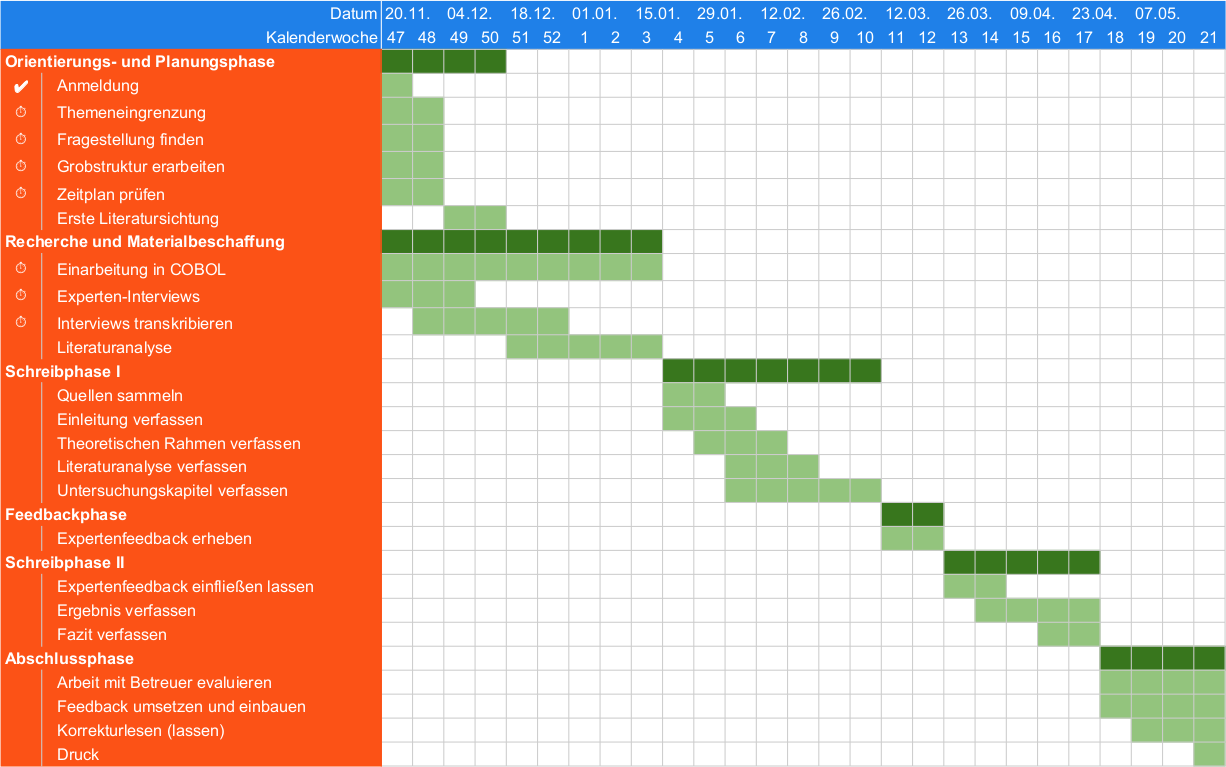
\includegraphics[width=0.25\textwidth]{Bilder/Zeitplan.PNG}
    \begin{tikzpicture}[node distance=0cm]
        \node (programRect) [inner sep=0pt, rectangle, draw, rounded corners, ultra thick, draw=black, fill=javaProgramm, minimum width=\linewidth, minimum height=.6\linewidth] at (0,0) {};
        \node[below = of programRect.north] () {COBOL Programm};

        \node (divisionRect) [inner sep=0pt, rectangle, draw, rounded corners, ultra thick, draw=black, fill=javaPackage!50!white, minimum width=.9\linewidth, minimum height=.5\linewidth] at (0,0) {};
        \node[below = of divisionRect.north] () {Divisions};

        \node (sectionRect) [inner sep=0pt, rectangle, draw, rounded corners, ultra thick, draw=black, fill=javaClass!50!white, minimum width=.5\linewidth, minimum height=.4\linewidth] at (-.15\linewidth,0) {};
        \node[below = of sectionRect.north] () {Sections};

        \node (paragraphRect) [inner sep=0pt, rectangle, draw, rounded corners, ultra thick, draw=black, fill=javaMethod!50!white, minimum width=.5\linewidth, minimum height=.3\linewidth] at (.15\linewidth,0) {};
        \node[below = of paragraphRect.north] () {Paragraphs};

        \node (sentenceRect) [inner sep=0pt, rectangle, draw, rounded corners, ultra thick, draw=black, fill=javaStatement!60!white, minimum width=.4\linewidth, minimum height=.2\linewidth] at (0,0) {};
        \node[below = of sentenceRect.north] () {Sentences};

        \node (statementRect) [inner sep=0pt, rectangle, draw, rounded corners, ultra thick, draw=black, fill=javaAnonClass!70!white, minimum width=.3\linewidth, minimum height=.1\linewidth] at (0,0) {};
        \node[below = of statementRect.north] () {Statements};

    \end{tikzpicture}
\caption{Strukturelle Bestandteile eines COBOL-Programms\label{cobolStructureDiagram}}
\end{wrapfigure}

Nebenstehende \autoref{cobolStructureDiagram} zeigt die strukturellen Bestandteile eines COBOL-Programms. 

Dabei gibt es folgende vier fest definierte \mintinline{cobolfree}{DIVISION}s:
\begin{itemize}
    \item \mintinline{cobolfree}{IDENTIFICATION DIVISION}
    \item \mintinline{cobolfree}{ENVIRONMENT DIVISION}
    \item \mintinline{cobolfree}{DATA DIVISION}
    \item \mintinline{cobolfree}{PROCEDURE DIVISION}
\end{itemize}


u.a. SENTENCE u. PARAGRAPH \& Statement und \{\}-Scope

-> DIVISIONS, SECTIONS, paragraphs, sentences, and statements, point

}